\newpage
\section{Design pattern utilizzati}


\subsection{Abstract Factory}
L'\textbf{\textit{Abstract Factory}} è un design pattern creazionale e fornisce un'interfaccia per creare famiglie di prodotti, senza dover esplicitare il nome concreto delle classi a cui si riferisce. In questo modo, si permette che un sistema sia indipendente dall'implementazione degli oggetti concreti e che il client, attraverso l'interfaccia, utilizzi diverse famiglie di prodotti. Quindi, il client conosce solo l’interfaccia per creare le famiglie di prodotti, ma non la sua implementazione concreta.
L’\textit{Abstract Factory} è costituito da 5 elementi:
\begin{itemize}
	\item \textbf{AbstractFactory}: dichiara un'interfaccia per le operazioni che crea oggetti product astratti;
	\item \textbf{ConcreteFactory}: implementa le operazioni per creare oggetti concreti product di AbstractProduct. Per garantire che nel sistema esiste un’unica istanza di ciascuna ConcreteFactory, è buona norma definire ciascuna di esse come \textit{Singleton};
	\item \textbf{AbstractProduct}: interfaccia che definisce la struttura base dei product che la factory può instanziare;
	\item \textbf{ConcreteProduct}: nel sistema possono essere creati n ConcreteProduct, ciascuno dei quali dovrà implementare l’interfaccia AbstractProduct;
	\item \textbf{Client}: utilizza l’AbstractFactory per generare i prodotti concreti all’interno del sistema.
\end{itemize}

\begin{figure}[H]
	\centering
	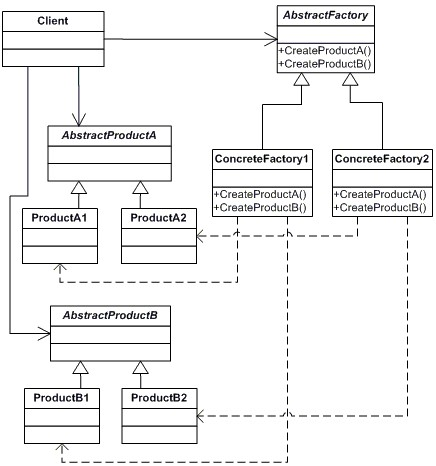
\includegraphics[width=0.5\linewidth]{IMG/abstract-pattern}
	\caption{Design pattern Abstract Factory}
\end{figure}

I punti di forza di questo design pattern sono:
\begin{itemize}
	\item Isola i client dall’implementazione delle classi concrete;
	\item Rafforza il raggruppamento di prodotti in famiglie;
	\item Rende possibile interscambiare facilmente le famiglie di prodotti, perché ogni factory concreta genera una famiglia di prodotti.
\end{itemize}


\subsection{Publish-Subscribe}
Il \textbf{\textit{Publish-Subscribe}} è un design pattern utilizzato per la comunicazione asincrona fra diversi processi, oggetti o altri agenti. I mittenti e i destinatari dialogano tramite data manager, definiti come Broker o Dispatcher, che svolgono la funzione di store-and-forward.
I mittenti (publisher) pubblicano i loro messaggi sui data manager, e i destinatari (subscriber) si rivolgono al data manager abbonandosi (subscribing) alla ricezione del messaggio a cui sono interessati. Per garantire un sistema scalabile, i publisher non sanno quanti e quali sono i subscriber, e viceversa. 
Con l'utilizzo del framework MeteorJS, la componente Broker o Dispatcher è completamente trasparente al programmatore, quindi, è necessario pubblicare i dati e abbonarsi ad essi, e MeteorJS si occuperà della comunicazione tra front-end e back-end.
\begin{figure}[H]
	\centering
	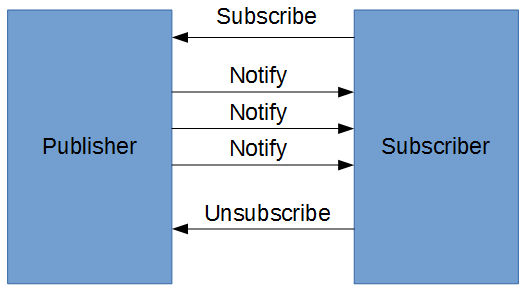
\includegraphics[width=0.5\linewidth]{IMG/pubsub}
	\caption{Design pattern Publish - Subscribe}
\end{figure}

I punti di forza di questo design pattern sono:
\begin{itemize}
	\item Totale disaccopiamento tra Publisher e Subscriber;
	\item Alta scalabilità nel software.
\end{itemize}


\subsection{Singleton}
Il \textbf{\textit{Singleton}} è un design pattern creazionale che ha lo scopo di garantire che venga creata una e una sola istanza di una determinata classe, e di fornire un punto di accesso globale a tale istanza.
Gli elementi caratteristici fondamentali per l'implementazione di questo pattern sono due:
\begin{itemize}
	\item un costruttore privato, per evitare che la classe possa essere istanziata arbitrariamente;
	\item un metodo statico per accedere alla singola istanza.
\end{itemize}
\begin{figure}[H]
	\centering
	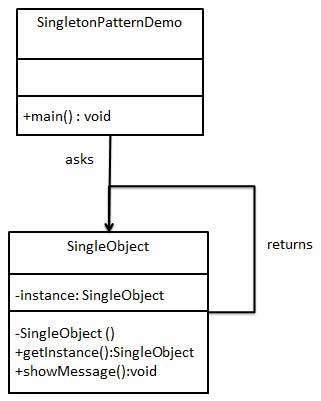
\includegraphics[width=0.4\linewidth]{IMG/singleton_pattern}
	\caption{Design pattern Singleton}
\end{figure}

I punti di forza di questo design pattern sono:
\begin{itemize}
	\item L'accesso controllato all'istanza;
	\item \MakeUppercase{è} possibile consentire più istanze, sempre in modo controllato.
\end{itemize}

